\chapter{\IfLanguageName{dutch}{Stand van zaken}{State of the art}}%
\label{ch:stand-van-zaken}
\addbibresource{bachproef.bib}            %% Bibliography file

% Tip: Begin elk hoofdstuk met een paragraaf inleiding die beschrijft hoe
% dit hoofdstuk past binnen het geheel van de bachelorproef. Geef in het
% bijzonder aan wat de link is met het vorige en volgende hoofdstuk.

% Pas na deze inleidende paragraaf komt de eerste sectiehoofding.

%Dit hoofdstuk bevat je literatuurstudie. De inhoud gaat verder op de inleiding, maar zal het onderwerp van de bachelorproef *diepgaand* uitspitten. De bedoeling is dat de lezer na lezing van dit hoofdstuk helemaal op de hoogte is van de huidige stand van zaken (state-of-the-art) in het onderzoeksdomein. Iemand die niet vertrouwd is met het onderwerp, weet nu voldoende om de rest van het verhaal te kunnen volgen, zonder dat die er nog andere informatie moet over opzoeken \autocite{Pollefliet2011}.
%
%Je verwijst bij elke bewering die je doet, vakterm die je introduceert, enz.\ naar je bronnen. In \LaTeX{} kan dat met het commando \texttt{$\backslash${textcite\{\}}} of \texttt{$\backslash${autocite\{\}}}. Als argument van het commando geef je de ``sleutel'' van een ``record'' in een bibliografische databank in het Bib\LaTeX{}-formaat (een tekstbestand). Als je expliciet naar de auteur verwijst in de zin (narratieve referentie), gebruik je \texttt{$\backslash${}textcite\{\}}. Soms is de auteursnaam niet expliciet een onderdeel van de zin, dan gebruik je \texttt{$\backslash${}autocite\{\}} (referentie tussen haakjes). Dit gebruik je bv.~bij een citaat, of om in het bijschrift van een overgenomen afbeelding, broncode, tabel, enz. te verwijzen naar de bron. In de volgende paragraaf een voorbeeld van elk.
%
%\textcite{Knuth1998} schreef een van de standaardwerken over sorteer- en zoekalgoritmen. Experten zijn het erover eens dat cloud computing een interessante opportuniteit vormen, zowel voor gebruikers als voor dienstverleners op vlak van informatietechnologie~\autocite{Creeger2009}.
%
%Let er ook op: het \texttt{cite}-commando voor de punt, dus binnen de zin. Je verwijst meteen naar een bron in de eerste zin die erop gebaseerd is, dus niet pas op het einde van een paragraaf.
%
%\lipsum[7-20]

\acrfull{ip} is het fundament van elk gestructureerd, goed functionerend en veilig netwerk. Het geeft de mogelijkheid efficiënt gegevens te routeren, netwerken te verdelen in meer beheersbare eenheden, toegang te beperken tot gevoelige data of systemen, services te identificeren en het oplossen van netwerkproblemen \autocite{Postel1981}. Dit hoofdstuk legt uit wat \acrfull{dns} en \acrfull{dhcp} is, waarom \acrshort{ipam} helpt bij het beheren van \acrshort{ip} netwerken en waarom \acrshort{http} nodig is om te communiceren met EIP. 

\subsection{DNS}
\textcite{Mockapetris1987} schrijft dat \acrshort{dns} een systeem is dat \textit{resource records} gebruikt om onder andere vertalingen te voorzien tussen domeinnamen en \acrshort{ip}-adressen. Als voorbeeld kan je via de browser naar google surfen via het \acrshort{ip}-adres \textit{142.251.36.35} of via domeinnaam \textit{www.google.be}.

Zoals beschreven door \textcite{Mockapetris1987} voorziet \acrshort{dns} meerdere types resource records die netwerkbeheerders kunnen meegeven: 
\begin{itemize}
    % TODO beschrijven wat een resource record is
    \item \textbf{A}: Dit resource record beschrijft een host adres. 
    Vb. \textit{”server1.voorbeeld.com. IN A 192.168.1.1”} maakt de vertaling zodat het toestel met de domeinnaam \textit{server1.voorbeeld.com} bereikbaar is zowel via het \acrshort{ip}-adres \textit{192.168.1.1} als via de domeinnaam. 
    \item \textbf{CNAME}: Dit resource record beschrijft de canonieke naam van een host, het wordt gebruikt om een alias of subdomein naar het hoofddomein door te verwijzen. Vb. \textit{"www.voorbeeld.com. IN CNAME server1.voorbeeld.com"} zorgt dat server1 ook bereikbaar is via "\textit{www.voorbeeld.com}".
    \item \textbf{MX}: Dit resource record is een \textit{mail exchange} record en wordt gebruikt om aan te geven welke mailservers verantwoordelijk zijn voor het ontvangen van mails binnen een domein. vb. \textit{"voorbeeld.com. IN MX 10 mailserver.voorbeeld.com"} geeft de \acrshort{dns} server mee welke server de mailserver is.
    \item \textbf{NS}: Dit resource record is een \textit{name server} record, het beschrijft welke \acrshort{dns}-servers verantwoordelijk zijn voor het beheren van \acrshort{dns}-informatie voor een domein. Vb. \textit{"voorbeeld.com. IN NS dns1.voorbeeld.com"} verwijst naar \textit{dns1} als \acrshort{dns}-server voor het domein “\textit{voorbeeld.com}”.
    \item \textbf{PTR}: Dit resource record is een \textit{Pointer} record, het wordt gebruikt om via \acrshort{ip} een vertaling te vragen aan de \acrshort{dns}-server in plaats van via de naam.
    \item \textbf{SOA}: Dit resource record is een \textit{Start of Authority} record die belangrijke informatie bevat over de zone, zoals welke de primaire \acrshort{dns}-server, contactpersonen, etc. zijn.
\end{itemize}

\subsection{DHCP}
Dit protocol voorziet een framework voor het doorgeven van configuratie-informatie naar hosts (lees: computers) op het netwerk . Zo kan een computer bijvoorbeeld een \acrshort{ip}-adres ontvangen waarmee die kan communiceren binnen het netwerk waarop die is aangesloten \autocite{Droms1997}.

\acrshort{ip}-netwerken worden door netwerkbeheerders op een logische manier opgesplitst in subnetwerken. Hierbij worden de beschikbare \acrshort{ip}-adressen verdeeld in subnetwerken (subnet). Toestellen binnen subnet A zullen elkaar kunnen bereiken terwijl een toestel in een subnet B zonder de nodige routering geen verbinding zal kunnen maken met de toestellen in subnet A.

Voor \acrshort{dhcp} zullen netwerkbeheerders subnets (of pools van \acrshort{ip}-adressen) aanbieden aan de \acrshort{dhcp}-server. Die zal gebruik maken van deze pools door (onder andere) \acrshort{ip}-adressen uit te delen aan toestellen die verbinden op het netwerk en daarbij de \acrshort{dhcp}-server laten weten dat ze nog geen \acrshort{ip}-adres hebben.

\textcite{Droms1997} schrijft dat \acrshort{dhcp} drie mechanismes gebruikt voor het uitdelen van \acrshort{ip}-adressen:
\begin{itemize}
    \item \textbf{Automatisch}: Permanent toewijzen van een \acrshort{ip}-adres.
    \item \textbf{Dynamisch}: \acrshort{ip}-adres voor een bepaalde tijd toewijzen.
    \item \textbf{Manueel}: Een (door de netwerkbeheerder) vooraf bepaald \acrshort{ip}-adres toewijzen, in vakjargon noemt met dit een \acrshort{ip}-reservatie.
\end{itemize}

\subsection{IPAM}
Naast de vele uitdagingen die zowel DNS als \acrshort{dhcp} met zich meebrengen, is het beheren van de beschikbare IP-adressen een belangrijk facet in het takenpakket van de netwerkbeheerder. \textcolor{purple}{Een slecht beheerd netwerk kan leiden tot \acrshort{ip}-conflicten waarbij meerdere apparaten hetzelfde \acrshort{ip}-adres gebruiken, wat op zijn beurt dan weer kan leiden tot netwerkstoringen en onvoorspelbaar gedrag van apparaten. Daarnaast zou men ook weinig tot geen overzicht hebben van de beschikbare IP-adressen en subnetten in het netwerk waardoor het moeilijker is om de beschikbare adressen te beheren en potentiële conflicten te identificeren.
    Een oplossing hiervoor is het toepassen van \acrshort{ipam}, dit is een systeem voor het beheren en toewijzen van \acrshort{ip}-adressen in een netwerk. Het biedt netwerkbeheerders een gestructureerde aanpak voor het beheren van \acrshort{ip}-adressen, waardoor ze een overzicht hebben van beschikbare en in gebruik zijnde adressen. IPAM kan ook helpen bij het vermijden van conflicten tussen subnetten en bij het bijhouden van de historie van \acrshort{ip}-adres toewijzingen.}

%Een mogelijke oplossing hiervoor is het gebruiken van \acrfull{ipam} via softwarepakketten die \acrshort{ipam} aanbieden.
%\acrshort{ipam} laat toe \acrshort{ip}-adressen efficiënt te beheren in een netwerk, het leidt tot een gestructureerde aanpak waardoor conflicten tussen subnetten worden vermeden. Het geeft een compleet overzicht van het netwerk met percentages van hoeveel adressen beschikbaar en in gebruik zijn. \acrshort{ipam} geeft eveneens de mogelijkheid om de historiek bij te houden waardoor het van pas komt voor schaalbaarheid en beveiliging van het netwerk \autocite{Rooney2020}.


\subsection{DNS, DHCP en IPAM}
\textcolor{purple}{De integratie van \acrshort{dns}, \acrshort{dhcp} en \acrshort{ipam} in een enkel systeem wordt vaak aangeduid als \acrfull{ddi}. \acrshort{ddi} biedt een benadering voor het beheren van de essentiële netwerkelementen die nodig zijn voor een goed functionerende infrastructuur. Door DNS, DHCP en IPAM te combineren, kunnen organisaties profiteren van een geïntegreerde aanpak voor het beheer van hun netwerkresources, waardoor efficiëntie en consistentie worden bevorderd.
    Zoals beschreven door \textcite{Fontein2023} leggen \acrshort{ddi}-applicaties doorgaans de focus voornamelijk op \acrshort{ipam}. Het zijn toepassingen die de beschikbare \acrshort{IP}-adressen en subnetten op een gestructureerde, overzichtelijke manier weergeven. Doorgaans is \acrshort{ddi} geïntegreerd met de \acrshort{dns}- en \acrshort{dhcp}-servers waardoor men deze componenten vanuit een centrale plek kunnen beheren. Er zijn meerdere \acrshort{ddi}-softwarepakketten ter beschikking die aangeboden worden door bedrijven zoals Solarwinds, Infoblox, en EfficientIP. Universiteit Gent heeft ervoor gekozen om EfficientIP aan te schaffen dus deze bachelorproef zal hier gebruik van maken voor het automatisch beheren van het netwerk.}

\subsection{Huidige werking Universiteit Gent}
\textcolor{purple}{Bij de aanvang van de bachelorproef is het netwerk van Universiteit Gent nog volledig beheert via subnetbestanden. Op basis van de logica van oud-werknemer Arsene Wauters werd een standaard bepaald en toegepast voor het nummeren en klasseren van subnetten, de zogenaamde ARWA-standaard (ARsene WAuters). Dankzij scripts worden deze subnetbestanden uitgelezen en wordt alle nodige informatie doorgegeven aan o.a. de \acrshort{dns}- en \acrshort{dhcp}-servers.}

\subsubsection{Subnetbestanden}
\textcolor{purple}{Op basis van ARWA-standaard krijgt elk subnetbestand een naam: “subnet” + “subnet klasse (A/B/C/D/G/I/N/P/T/V/W)” + “subnetnummer”, zo stelt bijvoorbeeld het subnetbestand “subnetB147.000” het subnet 157.193.147.0/24 voor. Deze ongecrypteerde tekstbestanden stellen elk een deel of een volledig subnet voor. Indien een subnet meer dan 254 beschikbare \acrshort{ip}-adressen bevat zullen er meerdere, opeenvolgende, subnetbestanden gebruikt worden.}
\begin{itemize}
    % TODO: Nakijken waarvoor OS key staat in host
    \item Header: Elk bestand begint met een “header” waarin belangrijke metadata beschreven staat over het netwerk: subnet klasse, nummer, naam, beschrijving, subnet masker, default gateway, DNS-servers, opties of DHCP, DNS, dot1x en security actief staan, datum van aanmaken, plaatsen waar het subnet actief is (via FI-codes), commentaar, en eventueel nog ACL-lijnen om extra toegang te voorzien aan het netwerk. Zie afbeelding \ref{fig:header}
    \item Hosts: Afhankelijk van de grootte van het subnet kunnen er tot 254 hosts beschreven staan in het bestand. Elke host, of die nu reeds bezet is of niet, staat beschreven in het subnetbestand. Hierbij krijg je dan via een key-value formaat, een opsomming van alle informatie: “N: hostnummer”, “H: hostnaam”, “E1: \acrshort{mac}" en eventueel “E2: extra \acrshort{mac}”, “T: beschrijving toestel”, “M: optie om veel mails te mogen versturen (voor bv. kopieerautomaten)”, “CS: type host, client of server”, “BO: Boot options (pad/naar/bootoption@server)”, “OS:  \textcolor{red}{???}”, ”P: en P#: locatie waar het toestel is aangesloten op het netwerk”, “CO: commentaar netwerkadmin”, ”V1-5: vakgroep universiteit + gegevens van het hoofd van de vakgroep”, “C1-5: gegevens van host contactpersoon”, “DC: datum van aanmaken registratie” en “DM: datum laatste wijziging”, optioneel kan er ook nog informatie bij geplaatst worden voor \acrshort{dns} A en CNAME resource records “AA: en CA:”, het openzetten van de beveiliging richting de host “S: en SI:” en ook extra mailinformatie “MD:”. Op de optionele informatie na staat deze informatie steeds voor elke host in het bestand. Indien een host \acrshort{IP} nog vrij is en ter beschikking staat voor een manuele reservatie dan zal dit worden weergegeven door een de opsomming van alle sleutelwaarden, met telkens een lege waarde. Afbeelding \ref{fig:host} toont een \acrshort{ip} registratie voor host stijnDemo, afbeelding \ref{fig:legeHost} geeft weer hoe een lege host is beschreven.
    []\item \end{itemize}
\begin{figure}[h!]
    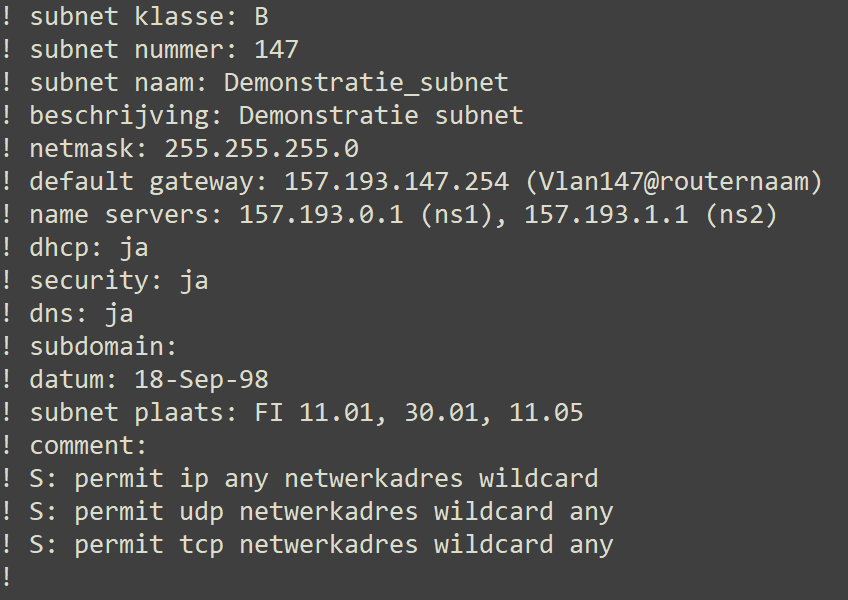
\includegraphics[scale=0.5]{header.png}
    \caption{header}
    \label{fig:header}
\end{figure}
\begin{figure}[h!]
    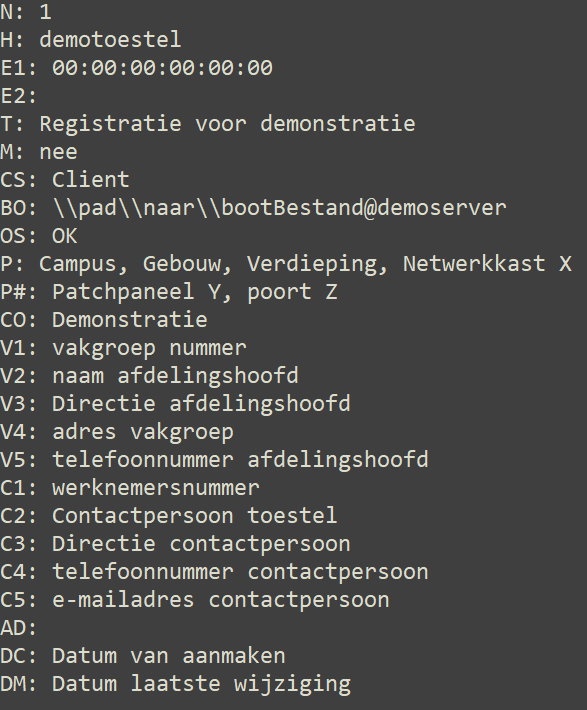
\includegraphics[scale=0.5]{host.png}
    \caption{host}
    \label{fig:host}
\end{figure}
\begin{figure}[h!]
    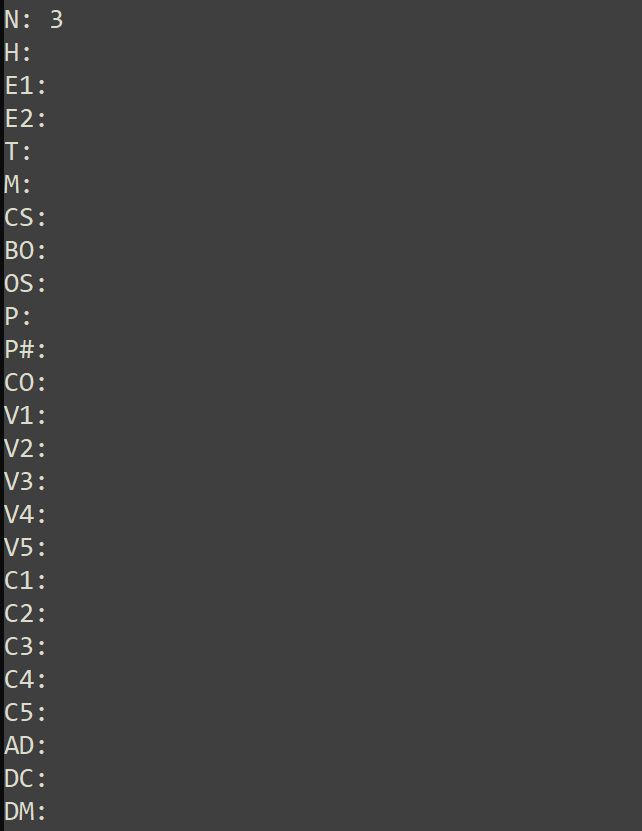
\includegraphics[scale=0.5]{legeHost.png}
    \caption{lege Host}
    \label{fig:legeHost}
\end{figure}

\subsubsection{IP registraties}
\textcolor{purple}{Via de interne webpagina www.netadmin.ugent.be 
}

\subsection{HTTP/HTTPS}
Om communicatie met de API van EIP mogelijk te maken wordt er gebruik gemaakt van \acrfull{http}. Dit is een client-serverprotocol die communicatie mogelijk maakt op het Internet. Zoals beschreven door \textcite{Fielding2014} maakt \acrshort{http} gebruik van \textit{Uniform Resource Identifiers (URI's)} om unieke web-resources te identificeren en biedt het verschillende methoden \textit{(GET, POST, PUT, DELETE)} waarmee clients acties kunnen uitvoeren op serverresources. \acrshort{http} is \textit{stateless}, elke aanvraag is onafhankelijk, en statuscodes zoals "200 OK"\ en \textit{headers} worden gebruikt om de resultaten en aanvullende informatie van serververzoeken aan te geven, waardoor een gestandaardiseerde communicatie tussen clients en servers mogelijk is.
Om deze informatieoverdracht te beveiligen, wordt \acrfull{https} gebruikt. \acrshort{https} bouwt voort op \acrshort{http}, maar voegt een extra beveiligingslaag toe door middel van \textit{Secure Sockets Layer (SSL)/Transport Layer Security (TLS)}-encryptie, waardoor de uitwisseling van gegevens tussen client en server wordt versleuteld. Hierdoor worden alle \acrshort{ip}-registraties en andere gegevens beter beschermd tegen potentiële aanvallen.
